% Rapport de projet -- compilation : pdflatex rapport.tex (deux fois)
\documentclass[11pt,a4paper]{article}

\usepackage{iftex}
\ifPDFTeX
  \usepackage[T1]{fontenc}
  \usepackage[utf8]{inputenc}
  \usepackage{lmodern}
\else                        % xelatex / tectonic : fontspec sert Latin Modern
  \usepackage{fontspec}      % par défaut, donc le même rendu qu'avec lmodern
\fi
\usepackage[french]{babel}
\usepackage{microtype}
\usepackage[margin=2.4cm]{geometry}
\usepackage{amsmath,amssymb}
\usepackage{booktabs}
\usepackage{graphicx}
\usepackage{xcolor}
\usepackage{caption}
\usepackage{listings}
\usepackage{fancyhdr}
\usepackage{url}
\usepackage[hidelinks]{hyperref}
\hypersetup{pdftitle={Mini-AlphaZero sur Puissance 4},
            pdfauthor={Amine Rouibi, Mohamed Zouad, Thomas Sinapi},
            pdfsubject={Recherche Monte-Carlo guidee par un reseau policy + value -- Universite Paris Dauphine-PSL}}

\graphicspath{{figures/}}
\captionsetup{font=small,labelfont=bf}
\setlength{\parskip}{0.3em}
\linespread{0.97}
\emergencystretch=3em

\pagestyle{fancy}
\fancyhf{}
\fancyhead[L]{\small Puissance 4 : UCT, RAVE et AlphaZero}
\fancyhead[R]{\small\thepage}
\renewcommand{\headrulewidth}{0.3pt}

\definecolor{codebg}{HTML}{F5F5F2}
\definecolor{codecm}{HTML}{52514E}
\lstdefinestyle{pseudo}{
  basicstyle=\ttfamily\small,
  commentstyle=\color{codecm}\itshape,
  backgroundcolor=\color{codebg},
  frame=single, framesep=5pt, rulecolor=\color{codecm!30},
  breaklines=true, columns=fullflexible, keepspaces=true, showstringspaces=false,
  numbers=left, numberstyle=\tiny\color{codecm}, xleftmargin=1.7em,
  literate={é}{{\'e}}1 {è}{{\`e}}1 {ê}{{\^e}}1 {à}{{\`a}}1 {ç}{{\c c}}1 {û}{{\^u}}1 {ô}{{\^o}}1 {î}{{\^i}}1 {œ}{{\oe}}1
}
\lstset{style=pseudo}

\newcommand{\pov}{\mathrm{pov}}

\title{\vspace{-1.5cm}\textbf{Mini-AlphaZero sur Puissance 4}\\[0.25em]
\large Recherche Monte-Carlo guidée par un réseau policy + value, entraîné par self-play}
\author{Amine Rouibi \and Mohamed Zouad \and Thomas Sinapi}
\date{Université Paris Dauphine -- PSL\\
Monte Carlo Search\\[0.3em]
\today}

\begin{document}
\maketitle
\thispagestyle{fancy}

\begin{abstract}
\noindent Nous implémentons, dans le périmètre du cours \emph{Monte Carlo Search},
la chaîne complète qui va du playout aléatoire à un AlphaZero miniature, sur le
Puissance 4 : moteur avec hachage de Zobrist et table de transposition, Flat Monte
Carlo, UCB à la racine, UCT récursif, AMAF / RAVE / GRAVE, alpha-bêta avec table de
transposition, puis réseau résiduel à deux têtes, PUCT, self-play parallélisé et
boucle d'entraînement. Trois des cinq critères fixés à l'avance sont atteints, dont
le critère décisif : à zéro simulation, la seule tête policy bat l'agent aléatoire
$93{,}8\,\%$ du temps. PUCT à $100$ simulations fait jeu égal avec UCT à $800$
playouts, ce qui chiffre l'apport du réseau à un facteur $8$ sur le budget de
recherche ; et le réseau redécouvre seul, par pur self-play et sans aucune
connaissance experte, que la colonne centrale est le meilleur coup d'ouverture --
un résultat connu du jeu résolu -- avec une probabilité de $0{,}914$. Les deux
critères manqués font l'objet d'un diagnostic complet : un premier entraînement a
échoué, et son analyse occupe la section~\ref{sec:discussion}.
\end{abstract}

\tableofcontents

\section{Introduction}\label{introduction}

\subsection{Pourquoi Monte-Carlo}\label{pourquoi-monte-carlo}

L'alpha-bêta suppose une bonne fonction d'évaluation. Aux échecs on en a une :
la valeur matérielle des pièces explique déjà l'essentiel de la position. Au Go
on n'en a pas, et c'est précisément le point de départ du cours : trente ans de
programmes de Go fondés sur la connaissance experte plafonnent au niveau
débutant, jusqu'à ce que \textbf{Gobble}~\cite{brugmann1993} propose de remplacer
l'évaluation par de l'\textbf{échantillonnage} --- jouer la partie au hasard jusqu'au
bout, un grand nombre de fois, et préférer le coup dont les parties aléatoires
finissent le mieux.

L'idée est contre-intuitive : les parties aléatoires sont d'une qualité
catastrophique. Mais leur \emph{moyenne} porte de l'information, et surtout elle ne
demande aucune connaissance du jeu. Quand on n'a pas de bonne fonction
d'évaluation, \textbf{échantillonner bat énumérer}.

Le cours suit ensuite l'enchaînement qui mène de là à AlphaGo Zero :

\begin{enumerate}
\def\labelenumi{\arabic{enumi}.}
\setlength{\itemsep}{1pt}\setlength{\parskip}{0pt}
\item
  \textbf{Flat Monte Carlo} --- répartir les playouts également entre les coups ;
\item
  \textbf{UCB à la racine} --- traiter le choix du coup comme un bandit manchot, et
  allouer les playouts là où ils sont informatifs ;
\item
  \textbf{UCT}~\cite{kocsis2006} --- appliquer UCB \emph{récursivement}, à chaque
  nœud de l'arbre ; c'est la rupture qui fait passer le Go de 10 kyu à 2 dan ;
\item
  \textbf{AMAF / RAVE / GRAVE} --- partager l'information entre coups pour accélérer
  la convergence quand les statistiques sont rares ;
\item
  \textbf{AlphaGo $\rightarrow$ AlphaGo Zero $\rightarrow$ AlphaZero} --- remplacer le playout aléatoire par
  un \textbf{réseau de neurones à deux têtes}, et remplacer le biais UCT par le
  \emph{prior} de la tête policy : c'est PUCT.
\end{enumerate}

\subsection{Ce que fait ce projet}\label{ce-que-fait-ce-projet}

Nous implémentons la transposition directe des slides \textbf{« Alpha Zero Project »}
et \textbf{« Projet Python »} du cours, qui décrivent le pipeline en cinq étapes pour
Breakthrough 5$\times$5 :

\begin{quote}
\begin{enumerate}
\def\labelenumi{\arabic{enumi})}
\setlength{\itemsep}{1pt}\setlength{\parskip}{0pt}
\item
  définir le réseau --- 2) implémenter PUCT avec le réseau --- 3) faire jouer
  l'algorithme contre lui-même --- 4) enregistrer les distributions Monte-Carlo et
  le résultat des parties --- 5) entraîner le réseau, puis itérer.
\end{enumerate}
\end{quote}

\textbf{Nous remplaçons Breakthrough 5$\times$5 par le Puissance 4}, pour des raisons de coût
de calcul : le facteur de branchement est de 7 au lieu d'environ 20, et les
parties sont plus courtes (21 coups en moyenne en jeu aléatoire, contre plusieurs
dizaines). Le pipeline, lui, est rigoureusement inchangé. Tout tourne sur CPU,
sur une machine à 8 cœurs.

\subsection{Critères de réussite et résultat global}\label{crituxe8res-de-ruxe9ussite-et-ruxe9sultat-global}

Les critères ont été fixés \textbf{avant} de lancer les expériences.
Voici le résultat final, mesuré sur le réseau final avec 100 simulations :

\begin{table}[htbp]
\centering\small
\caption{Critères de réussite, fixés avant les expériences et mesurés sur le réseau final à 100 simulations.}
\label{tab:criteres}
\setlength{\tabcolsep}{4pt}
\begin{tabular}{@{}lllccc@{}}
\toprule
\textbf{Critère} & \textbf{Seuil} & \textbf{Mesuré} & \textbf{IC Wilson 95 \%} & \textbf{parties} & \textbf{Atteint} \\
\midrule
C1 --- PUCT vs Aléatoire & 98,0 \% & \textbf{100,0 \%} & {[}93,6 \%, 100,0 \%{]} & 56 & \textbf{oui} \\
C2 --- PUCT vs UCT (100) & 70,0 \% & \textbf{61,6 \%} & {[}48,5 \%, 73,2 \%{]} & 56 & non \\
C3 --- PUCT vs alpha-bêta d.4 & 60,0 \% & \textbf{53,1 \%} & {[}43,3 \%, 62,6 \%{]} & 98 & non \\
C4 --- Réseau seul vs Aléatoire & 85,0 \% & \textbf{93,8 \%} & {[}84,2 \%, 97,7 \%{]} & 56 & \textbf{oui} \\
C5 --- pertes décroissantes & qualitatif & \multicolumn{3}{l}{2,29 $\rightarrow$ 1,68 sur 14 itérations} & \textbf{oui} \\
\bottomrule
\end{tabular}
\end{table}

\textbf{Trois critères sur cinq sont atteints.} C2 et C3 ne le sont pas, mais leurs
intervalles de confiance à 95 \% contiennent le seuil visé (70 \% $\in$ {[}48,5 ; 73,2{]} et
60 \% $\in$ {[}43,3 ; 62,6{]}) : avec le nombre de parties dont nous disposons, nous ne
pouvons pas conclure que le seuil est manqué, seulement que nous ne pouvons pas
démontrer qu'il est atteint. La §8 leur est consacrée, et s'appuie sur un
\textbf{premier run raté} que nous rapportons intégralement.

C4 est le critère décisif : C1 à C3 pourraient passer avec un réseau nul mais une
recherche correcte ; \textbf{seul C4 prouve que le réseau a appris quelque chose},
puisqu'il mesure la politique seule, à zéro simulation. Il est atteint largement.

\section{Le jeu et sa modélisation}\label{le-jeu-et-sa-moduxe9lisation}

\paragraph{Le jeu :}

Grille de 6 lignes et 7 colonnes. Chaque joueur pose à tour de rôle un pion dans
une colonne, où il tombe sur la première case libre. Le premier qui aligne quatre
pions (horizontalement, verticalement ou en diagonale) gagne ; si les 42 cases
sont remplies sans alignement, la partie est nulle.

Deux propriétés comptent pour nous :

\begin{itemize}
\setlength{\itemsep}{1pt}\setlength{\parskip}{0pt}
\item
  \textbf{Le facteur de branchement est 7 au maximum}, et décroît quand les colonnes
  se remplissent. C'est très inférieur au Go ($\approx$ 250) ou à Breakthrough 5$\times$5. La
  recherche couvre donc beaucoup de terrain avec peu de simulations.
\item
  \textbf{Le jeu est résolu}~\cite{allis1988,allen1989} : avec un jeu parfait, \textbf{le
  premier joueur gagne}, en jouant la colonne centrale au premier coup. Cette
  propriété a deux conséquences directes sur ce rapport : d'une part elle impose
  le protocole d'ouvertures équilibrées de la §6, sans quoi tous les chiffres
  seraient faussés ; d'autre part elle nous donne une vérité terrain gratuite
  pour l'expérience E7.
\end{itemize}

Mesure de contrôle du moteur : sur 5 000 parties aléatoires, JAUNE gagne 2 825
fois, ROUGE 2 161 fois, et 14 parties sont nulles. L'avantage du premier joueur
est donc déjà visible en jeu purement aléatoire.

\paragraph{Représentation et interface :}

Nous suivons le style du cours : une classe \texttt{Board} avec \texttt{legalMoves}, \texttt{play},
\texttt{terminal}, \texttt{score} et \texttt{playout} (section Breakthrough).

\begin{lstlisting}[caption={L'état de jeu.},label={lst:board}]
ROWS, COLS = 6, 7
EMPTY, YELLOW, RED = 0, 1, 2      # YELLOW joue en premier

class Board:
    cells:   list[int]    # 42 cases, index = row*7 + col, ligne 0 = BAS
    heights: list[int]    # 7 hauteurs de colonne
    turn:    int
    moves:   int
    h:       int          # hash de Zobrist
    last:    tuple | None # (ligne, colonne) du dernier coup
    winner:  int | None
\end{lstlisting}

\textbf{Convention de score.} \texttt{score()} renvoie une valeur dans \texttt{{[}0,\ 1{]}} \textbf{du point de
vue de JAUNE} : \texttt{1.0} si JAUNE gagne, \texttt{0.0} si ROUGE gagne, \texttt{0.5} pour une nulle.
C'est exactement la convention du cours (\texttt{1.0\ if\ White\ wins,\ 0.0\ else,\ 0.5\ draw}), et nous l'avons conservée telle quelle pour pouvoir transcrire sans
adaptation les codes UCT, RAVE, GRAVE et PUCT du cours, y compris l'idiome
\texttt{if\ board.turn\ ==\ RED:\ Q\ =\ 1\ -\ Q}, qui revient dans les quatre
algorithmes.

\textbf{Détection de victoire incrémentale.} Après chaque coup, on ne teste que les
alignements passant par la dernière case remplie. Nous précalculons, pour chacune
des 42 cases, la liste des alignements de 4 qui la contiennent (69 alignements au
total sur la grille) ; le test est alors une boucle sur environ 6,6 alignements.
C'est O(1) par coup.

\textbf{Ordre des coups.} \texttt{legalMoves()} renvoie les colonnes dans l'ordre
\texttt{{[}3,\ 2,\ 4,\ 1,\ 5,\ 0,\ 6{]}} --- le centre d'abord, comme le recommande le cours pour
l'ordonnancement alpha-bêta. Tous les agents départagent donc les ex æquo de la
même manière, ce qui rend les comparaisons plus propres.

\paragraph{Hachage de Zobrist~\cite{zobrist1970} et table de transposition :}

Le cours pose la question : \textbf{combien de nombres aléatoires faut-il ?} Un par
couple (couleur, case), plus un pour le trait :

\begin{equation*}
2 \times 42 + 1 = 85 \text{ entiers de 64 bits.}
\end{equation*}

C'est beaucoup moins que les 789 nombres que le cours compte pour les échecs
(6 pièces $\times$ 2 couleurs $\times$ 64 cases, plus le trait et les droits de roque) --- parce
qu'il n'y a ici qu'un seul type de pièce et 42 cases.

\texttt{play()} met à jour le hash exactement comme le code du cours, en XOR-ant
dans \texttt{self.h} les deux nombres \texttt{ZOBRIST[player-1][idx]} et
\texttt{ZOBRIST\_TURN}.
Les nombres sont tirés à partir d'une \textbf{graine fixe}, ce qui est indispensable
ici : le self-play est multi-processus et tous les workers doivent s'accorder sur
les hashs.

Vérifications :

\begin{itemize}
\setlength{\itemsep}{1pt}\setlength{\parskip}{0pt}
\item
  le hash maintenu par XOR est identique au hash recalculé de zéro, sur les
  63 464 coups de 3 000 parties ;
\item
  \textbf{zéro collision sur 200 012 positions distinctes}, ce qui est attendu dans un
  espace de $2^{64}$ ;
\item
  deux ordres de coups différents menant à la même position partagent bien la
  même entrée (\texttt{{[}0,1,2,3{]}} et \texttt{{[}2,3,0,1{]}}). Notons au passage qu'il faut
  \textbf{quatre} coups pour transposer au Puissance 4 : \texttt{{[}3,2{]}} et \texttt{{[}2,3{]}} donnent aux
  deux couleurs des cases opposées, ce ne sont pas les mêmes positions.
\end{itemize}

La table de transposition est un \texttt{dict{[}int,\ Entry{]}} indexé par \texttt{board.h},
réinitialisé à chaque coup joué à la racine --- exactement le \texttt{Table\ =\ \{\}} du
\texttt{BestMoveUCT} du cours. La disposition de l'entrée reprend la liste du cours :

\begin{lstlisting}[caption={Disposition d'une entrée de la table de transposition.},label={lst:entry}]
class Entry:
    n:         float          # t[0]  playouts totaux
    nplayouts: np.ndarray(7)  # t[1]  playouts par coup
    nwins:     np.ndarray(7)  # t[2]  victoires par coup
    namaf:     np.ndarray(84) # t[3]  playouts AMAF   (RAVE / GRAVE)
    wamaf:     np.ndarray(84) # t[4]  victoires AMAF
    prior:     np.ndarray(7)  # PUCT : tête policy
    value:     float          # PUCT : tête value
\end{lstlisting}

\textbf{Taux de hit mesuré} (E9) : 77,5 \% pour UCT, 82,6 \% pour GRAVE, 78,4 \% pour
PUCT. Autrement dit, dans plus de trois descentes sur quatre, la position
atteinte est déjà connue de la table. Le Puissance 4 est effectivement très riche
en transpositions, puisque toute permutation de l'ordre des colonnes jouées mène
à la même position. L'alpha-bêta n'affiche que 13,2 \% parce qu'il explore un
arbre beaucoup plus étroit, fortement élagué.

\paragraph{Codes de coups pour AMAF :}

Pour AMAF il faut un « code » identifiant un coup indépendamment du moment où il
est joué. Le choix naïf serait \textbf{la colonne} : 7 codes. Nous ne l'avons pas
retenu, et c'est délibéré.

Un playout de Puissance 4 dure une vingtaine de coups et joue donc \textbf{presque
toutes les colonnes}. Avec 7 codes seulement, chaque code serait crédité dans
presque chaque playout, les statistiques AMAF de tous les coups convergeraient
vers la même valeur, et l'heuristique n'apporterait aucun signal.

Nous codons donc \textbf{la case remplie et le joueur} :

\begin{equation*}
\mathrm{code} \;=\; \mathrm{joueur} \times 42 \;+\; \mathrm{ligne} \times 7 \;+\; \mathrm{colonne}
\qquad\text{soit } 84 \text{ codes.}
\end{equation*}

C'est l'analogue direct du \texttt{Move.code} du cours pour Breakthrough
(\texttt{5*(Dy*x1+y1)+direction}, dédoublé par couleur) : le code identifie \emph{où} le coup
atterrit, pas seulement \emph{dans quelle direction} on le joue. Deux pions de la même
couleur dans la même colonne mais à des hauteurs différentes sont des coups
différents, ce qui est exactement la sémantique voulue.

\section{Recherche Monte-Carlo sans réseau}\label{recherche-monte-carlo-sans-ruxe9seau}

Nous avons implémenté les quatre premiers barreaux de l'échelle du cours, dans
l'ordre, en transcrivant les extraits de code des slides.

\subsection{Playout et Flat Monte Carlo}\label{playout-et-flat-monte-carlo}

Le playout est uniforme et joue jusqu'à une position terminale. \texttt{flat(board,\ n)}
répartit les \texttt{n} playouts également entre les coups légaux et renvoie le coup de
meilleure moyenne.

\subsection{UCB à la racine}\label{ucb-uxe0-la-racine}

\texttt{UCB(board,\ n)} traite la racine comme un bandit à 7 bras et alloue chaque
playout au coup maximisant

\begin{equation*}
\bar{X}_i \;+\; c\,\sqrt{\frac{\ln i}{n_i}}
\end{equation*}

C'est le dilemme exploration / exploitation du cours : exploiter le bras qui
semble le meilleur, mais explorer assez pour ne pas rester sur une illusion
statistique.

\subsection{UCT}\label{uct}

\texttt{UCT(board)} applique la même règle \textbf{récursivement} à chaque nœud, avec la table
de transposition. Nous reprenons le code du cours tel quel :

\begin{lstlisting}[caption={Le cœur de UCT, transcrit du cours.},label={lst:uct}]
def UCT(board, table, c=0.4):
    if board.terminal():
        return board.score()
    t = table.look(board)
    if t is not None:
        for m in board.legalMoves():
            ni = t.nplayouts[m]
            if ni == 0:
                val = INF                       # tout coup est essayé une fois
            else:
                Q = t.nwins[m] / ni
                if board.turn == RED:
                    Q = 1.0 - Q                 # convention du cours
                val = Q + c * sqrt(log(t.n) / ni)
            ...
        board.play(best)
        res = UCT(board, table, c)              # récursion
        t.n += 1; t.nplayouts[best] += 1; t.nwins[best] += res
        return res
    table.add(board)
    return board.playout()                      # expansion + simulation
\end{lstlisting}

Deux écarts, purement notationnels : l'entrée est un petit objet plutôt qu'une
liste (\texttt{t.n} pour \texttt{t{[}0{]}}), et les tableaux par coup sont indexés par \textbf{colonne}
plutôt que par rang dans \texttt{legalMoves()} --- au Puissance 4, le coup \emph{est} la
colonne, et les tableaux font déjà 7 cases.

Un détail qui a son importance pour lire les chiffres : \textbf{la première simulation
ne fait que créer la racine} et jouer un playout, sans rien incrémenter. Après
\texttt{n} simulations, la racine totalise donc \texttt{n\ -\ 1} visites.

\subsection{Résultats : l'échelle du cours (E1)}\label{ruxe9sultats-luxe9chelle-du-cours-e1}

Toutes à 200 playouts, 56 parties à ouvertures équilibrées par confrontation.

\begin{table}[htbp]
\centering\small
\caption{E1 --- l'échelle du cours à 200 playouts, en confrontation deux à deux (56 parties à ouvertures équilibrées par ligne).}
\label{tab:e1}
\setlength{\tabcolsep}{5pt}
\begin{tabular}{@{}llccrr@{}}
\toprule
\textbf{A} & \textbf{B} & \textbf{victoire de A} & \textbf{IC Wilson 95 \%} & \textbf{V/N/D} & \textbf{Elo} \\
\midrule
Aléatoire & Flat MC (200) & 5,4 \% & {[}1,8 \%, 14,6 \%{]} & 3/0/53 & --499 \\
Aléatoire & UCB racine (200) & 0,0 \% & {[}0,0 \%, 6,4 \%{]} & 0/0/56 & --3600 \\
Aléatoire & UCT (200) & 0,0 \% & {[}0,0 \%, 6,4 \%{]} & 0/0/56 & --3600 \\
Flat MC (200) & UCB racine (200) & 58,0 \% & {[}45,0 \%, 70,0 \%{]} & 31/3/22 & +56 \\
Flat MC (200) & UCT (200) & 25,9 \% & {[}16,2 \%, 38,6 \%{]} & 14/1/41 & --183 \\
UCB racine (200) & UCT (200) & 32,1 \% & {[}21,4 \%, 45,2 \%{]} & 17/2/37 & --130 \\
\bottomrule
\end{tabular}
\end{table}

La progression du cours est nette : n'importe quelle méthode Monte-Carlo écrase
l'aléatoire, et \textbf{UCT domine largement les deux méthodes qui n'explorent qu'à la
racine} (74,1 \% contre Flat MC, 67,9 \% contre UCB). En revanche Flat MC et UCB
sont statistiquement indiscernables ici (58,0 \%, IC {[}45,0 ; 70,0{]} qui contient
50 \%). Ce n'est pas surprenant à 200 playouts et 7 coups : allouer intelligemment
28 playouts par coup ne change pas grand-chose ; ce qui change tout, c'est de
descendre dans l'arbre.

\subsection{Où la différence se joue vraiment}\label{ouxf9-la-diffuxe9rence-se-joue-vraiment}

Une mesure complémentaire éclaire ce résultat. Sur
30 positions où le joueur au trait a un \textbf{gain immédiat}, et 30 positions où il
doit \textbf{parer une menace immédiate} sous peine de perdre au coup suivant :

\begin{table}[htbp]
\centering\small
\caption{Tactique élémentaire : gains immédiats pris et pertes immédiates parées, sur 30 positions de chaque type, selon le budget.}
\label{tab:tactique}
\begin{tabular}{@{}lcccc@{}}
\toprule
& \textbf{gains pris} & \multicolumn{3}{c}{\textbf{parades /30}} \\
\cmidrule(l){3-5}
\textbf{algorithme} & \textbf{/30} & \textbf{200} & \textbf{400} & \textbf{1000} \\
\midrule
Flat MC & 30 & 23 & 26 & 28 \\
UCB racine & 30 & 26 & 26 & 27 \\
UCT & 30 & 29 & 29 & \textbf{30} \\
GRAVE & 30 & 29 & \textbf{30} & \textbf{30} \\
RAVE & 30 & \textbf{30} & \textbf{30} & \textbf{30} \\
PUCT & 30 & \textbf{30} & \textbf{30} & \textbf{30} \\
\bottomrule
\end{tabular}
\end{table}

Tous les algorithmes prennent un gain immédiat sans exception : il suffit d'un
playout pour voir la partie se terminer sur une victoire. \textbf{Parer est beaucoup
plus difficile pour les méthodes de racine}, et la raison est instructive : ne
pas parer rapporte quand même environ 0,5 en playout aléatoire, parce qu'un
adversaire aléatoire oublie très souvent de punir. Avec 200/7 = 28 playouts par
coup, cette différence se noie dans le bruit. Seule une recherche en arbre, qui
concentre son budget là où c'est décisif, la résout --- et UCT atteint 30/30 dès
qu'on lui donne 1 000 playouts. C'est exactement la raison pour laquelle UCT bat
Flat MC dans le tableau E1.

\subsection{Constante d'exploration (E2)}\label{constante-dexploration-e2}

\begin{figure}[htbp]
\centering
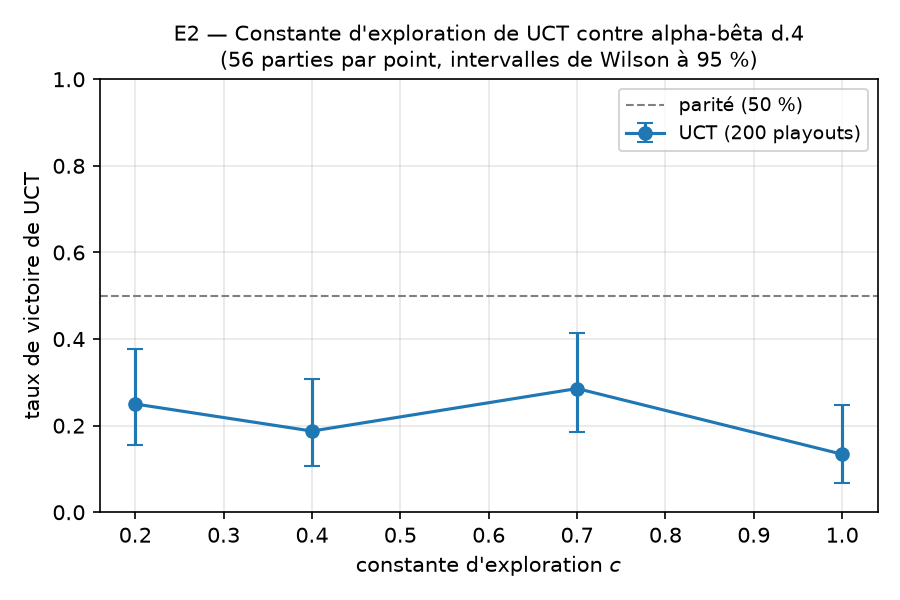
\includegraphics[width=0.44\linewidth]{figures/fig_E2_constante_exploration.png}
\caption{E2 --- Constante d'exploration de UCT contre l'alpha-bêta de profondeur 4, 56 parties par point, intervalles de Wilson à 95 \%.}
\end{figure}

Sur la grille \texttt{\{0,2\ ;\ 0,4\ ;\ 0,7\ ;\ 1,0\}} contre l'alpha-bêta de profondeur 4, les
scores sont respectivement 25,0 \%, 18,8 \%, 28,6 \% et 13,4 \%. \textbf{Les intervalles de
confiance se recouvrent tous largement} sauf pour \texttt{c\ =\ 1,0}, nettement moins bon.
Nous ne pouvons donc pas départager 0,2, 0,4 et 0,7 avec 56 parties ; on observe
seulement que trop explorer nuit clairement. Nous conservons \textbf{\texttt{c\ =\ 0,4}}, la
valeur du cours, qui est bien calibrée pour des scores dans \texttt{{[}0,\ 1{]}} --- et nous
notons honnêtement que nos mesures ne la valident pas contre 0,2 ou 0,7, elles
n'ont simplement pas la puissance statistique pour le faire.

\subsection{AMAF, RAVE et GRAVE (E8)}\label{amaf-rave-et-grave-e8}

Nous avons transcrit \texttt{playoutAMAF}, \texttt{updateAMAF}, \texttt{RAVE} et \texttt{GRAVE(board,\ played,\ tref)} du cours. \texttt{updateAMAF} ne crédite que la \textbf{première occurrence} de
chaque code dans le playout. Le poids de mélange est celui du cours~\cite{gelly2007} :

\begin{equation*}
\beta \;=\; \frac{n_{\mathrm{AMAF}}}{n_i + n_{\mathrm{AMAF}} + b\,n_i\,n_{\mathrm{AMAF}}},
\qquad b = 10^{-5}
\end{equation*}

GRAVE~\cite{cazenave2015grave} utilise les statistiques AMAF du \textbf{plus proche ancêtre ayant au moins \texttt{ref}
playouts} (\texttt{ref\ =\ 50} comme dans le cours). Avec \texttt{ref\ =\ 0}, chaque nœud est son
propre référent et GRAVE redevient RAVE : c'est notre \textbf{vérification de
cohérence}, et elle passe --- sur 25 positions et 300 playouts, à graine fixée, GRAVE(ref=0) et
RAVE produisent \textbf{exactement} la même distribution de visites.

\begin{table}[htbp]
\centering\small
\caption{E8 --- UCT, RAVE et GRAVE ($\mathrm{ref} = 50$) à 200 et 1000 playouts.}
\label{tab:e8}
\begin{tabular}{@{}lllll@{}}
\toprule
budget & confrontation & victoire de A & IC Wilson 95 \% & V/N/D \\
\midrule
200 & GRAVE vs UCT & 53,6 \% & {[}40,7 \%, 66,0 \%{]} & 29/2/25 \\
200 & RAVE vs UCT & 49,1 \% & {[}36,5 \%, 61,8 \%{]} & 26/3/27 \\
200 & GRAVE vs RAVE & 49,1 \% & {[}36,5 \%, 61,8 \%{]} & 27/1/28 \\
1000 & GRAVE vs UCT & 35,7 \% & {[}24,5 \%, 48,8 \%{]} & 18/4/34 \\
1000 & RAVE vs UCT & 47,3 \% & {[}34,8 \%, 60,1 \%{]} & 25/3/28 \\
1000 & GRAVE vs RAVE & 47,3 \% & {[}34,8 \%, 60,1 \%{]} & 24/5/27 \\
\bottomrule
\end{tabular}
\end{table}

\textbf{C'est un résultat négatif.} À 200 playouts, GRAVE, RAVE et UCT sont indiscernables (tous les IC contiennent
50 \%). À 1 000 playouts, \textbf{GRAVE devient significativement moins bon que UCT}
(35,7 \%, IC {[}24,5 ; 48,8{]} --- la borne haute reste sous 50 \%).

L'explication tient à l'hypothèse même d'AMAF : \emph{la valeur d'un coup dépend peu du
moment où il est joué}. Cette hypothèse est raisonnable au Go, où une pierre
posée sur une intersection y reste et garde à peu près la même fonction. \textbf{Elle
est beaucoup plus faible au Puissance 4}, pour une raison structurelle : une case
n'est jouable qu'à une hauteur donnée, et seulement quand toutes les cases en
dessous sont remplies. Jouer la case (3, 4) « plus tard dans le playout » n'est
pas le même coup que la jouer maintenant --- c'est un coup qui n'était même pas
légal au moment où on l'évalue. Le crédit AMAF mélange donc des situations qui ne
sont pas comparables, et introduit un biais que les vraies statistiques doivent
ensuite corriger. Plus le budget augmente, plus les vraies statistiques
deviendraient fiables toutes seules, et plus le biais AMAF résiduel coûte cher :
d'où la dégradation entre 200 et 1 000 playouts.

S'ajoute un coût pratique : GRAVE prend \textbf{27,2 ms par coup contre 8,1 ms pour
UCT} à budget égal (E9), soit plus de trois fois plus, à cause de la mise à jour
des tableaux de 84 codes à chaque playout. À temps égal plutôt qu'à playouts égaux,
le verdict serait encore plus défavorable.

\section{De AlphaGo à AlphaZero}\label{de-alphago-uxe0-alphazero}

\subsection{Les quatre réseaux d'AlphaGo}\label{les-quatre-ruxe9seaux-dalphago}

Le cours décrit AlphaGo~\cite{silver2016} comme la combinaison de quatre réseaux : une
\emph{policy} supervisée apprise sur des parties de joueurs forts, une \emph{policy} rapide
pour les playouts, une \emph{policy} raffinée par apprentissage par renforcement, et
un réseau de \emph{value}. La recherche combine la valeur du réseau et le résultat
d'un playout guidé.

\subsection{AlphaGo Zero : ce qui est retiré}\label{alphago-zero-ce-qui-est-retiruxe9}

AlphaGo Zero~\cite{silver2017} est surtout remarquable par ce qu'il \textbf{supprime} :

\begin{itemize}
\setlength{\itemsep}{1pt}\setlength{\parskip}{0pt}
\item
  plus de parties humaines : uniquement du self-play depuis l'initialisation
  aléatoire ;
\item
  plus de connaissance experte en entrée : le plateau brut ;
\item
  plus de playout du tout : la valeur de la feuille est donnée par la \textbf{tête
  value} ;
\item
  un seul réseau \textbf{à deux têtes} (policy et value) partageant une tour
  résiduelle.
\end{itemize}

La recherche devient \textbf{PUCT} : le terme d'exploration d'UCT est remplacé par un
terme proportionnel au \emph{prior} donné par la tête policy.

\subsection{PUCT}\label{puct}

Le cours donne la formule de sélection~\cite{rosin2011puct} :

\begin{equation*}
\mathrm{val}(a) \;=\; Q(s,a) \;+\; c_{\mathrm{puct}}\,P(a \mid s)\,
\frac{\sqrt{N(s)}}{1 + N(s,a)}
\end{equation*}

et précise que le \texttt{Q} d'un coup \textbf{non visité} vaut la \textbf{valeur réseau du nœud}
(le \texttt{Q\ =\ t{[}4{]}} du code du cours). Notre transcription :

\begin{lstlisting}[caption={PUCT : la même récursion, guidée par le réseau.},label={lst:puct}]
def PUCT(board, table, net, c_puct=1.0):
    if board.terminal():
        return board.score()
    t = table.look(board)
    if t is None:                       # feuille : PAS de playout
        _, value = expand(board, table, net)
        return value                    # la tête value remplace le rollout
    for m in board.legalMoves():
        ni = t.nplayouts[m]
        Q = (t.nwins[m] / ni) if ni > 0 else t.value
        if board.turn == RED:
            Q = 1.0 - Q                 # toujours la convention du cours
        val = Q + c_puct * t.prior[m] * sqrt(t.n) / (1.0 + ni)
        ...
    board.play(best)
    res = PUCT(board, table, net, c_puct)
    t.n += 1; t.nplayouts[best] += 1; t.nwins[best] += res
    return res
\end{lstlisting}

La structure récursive est \textbf{identique} à celle d'UCT. Trois choses seulement
changent, et ce sont exactement les trois que le cours attribue à AlphaGo Zero :

\begin{enumerate}
\def\labelenumi{\arabic{enumi}.}
\setlength{\itemsep}{1pt}\setlength{\parskip}{0pt}
\item
  la formule de sélection utilise le prior au lieu de $\sqrt{\ln n / n_i}$ ;
\item
  la feuille est évaluée par le réseau, \textbf{il n'y a plus aucun playout} ;
\item
  à la racine, \textbf{et uniquement en self-play}, les priors sont mélangés à un
  bruit de Dirichlet : $P \leftarrow 0{,}75\,P + 0{,}25\,\mathrm{Dir}(1{,}0)$.
  Les coups illégaux sont masqués avant le softmax.
\end{enumerate}

\texttt{c\_puct\ =\ 1,0} par défaut, ce qui est cohérent avec une échelle de valeurs dans
\texttt{{[}0,\ 1{]}}.

\subsection{Notre transposition au Puissance 4}\label{notre-transposition-au-puissance-4}

Le pipeline est celui des slides, sans modification : self-play avec PUCT $\rightarrow$
échantillons (état, distribution de visites, résultat) $\rightarrow$ entraînement $\rightarrow$ itération.
Nous ne gardons \textbf{pas d'arène de sélection} (le \emph{gating} d'AlphaGo Zero) : comme
AlphaZero~\cite{silver2018}, on conserve toujours le dernier réseau. C'est plus simple et plus
rapide, et sur 14 itérations les parties d'arène coûteraient plus cher qu'elles ne
rapporteraient.

\section{Implémentation}\label{impluxe9mentation}

Tous les agents --- aléatoire, Flat MC, UCB, UCT, RAVE, GRAVE, alpha-bêta et PUCT ---
exposent la même interface : ils reçoivent une position et renvoient un coup,
accompagné des compteurs qui alimentent toutes les mesures de ce rapport
(distribution de visites, priors et value du réseau, temps par coup, hits de la
table de transposition). C'est ce qui rend les confrontations de la §7 comparables :
les agents ne diffèrent que par la manière de choisir le coup.

\subsection{Encodage}\label{encodage}

Trois plans de 6$\times$7 en \texttt{float32}, \textbf{du point de vue du joueur au trait} --- le
cours écrit « rotate the board for white so that moves are always forward », et le
slide « Projet Python » demande exactement trois matrices pour Breakthrough :

\begin{enumerate}
\def\labelenumi{\arabic{enumi}.}
\setlength{\itemsep}{1pt}\setlength{\parskip}{0pt}
\item
  les pions du joueur au trait,
\item
  les pions de l'adversaire,
\item
  un plan constant à 1,0.
\end{enumerate}

Le réseau n'a donc jamais besoin de savoir quelle couleur il joue.

\subsection{Réseau}\label{ruxe9seau}

\begin{lstlisting}[caption={La tour résiduelle et ses deux têtes.},label={lst:net},numbers=none]
entrée (3, 6, 7)
  -> Conv3x3(64) + BN + ReLU
  -> 3 x BlocRésiduel(64)
  -> tête policy : Conv1x1(2) + BN + ReLU -> aplatir -> Linear(7)   [logits]
  -> tête value  : Conv1x1(1) + BN + ReLU -> aplatir -> Linear(32)
                  -> ReLU -> Linear(1) -> tanh
\end{lstlisting}

\textbf{226 010 paramètres.} La passe avant sur un exemple coûte de l'ordre de la
milliseconde sur CPU (1,08 ms mesuré pour l'agent « réseau seul », E9).

La perte est celle d'AlphaGo Zero~\cite{silver2017}, citée par le cours :

\begin{equation*}
L \;=\; \underbrace{-\sum_a \pi(a)\,\log p_\theta(a)}_{\text{entropie croisée (policy)}}
\;+\; \underbrace{\bigl(v_\theta - z\bigr)^2}_{\text{MSE (value)}}
\;+\; \underbrace{10^{-4}\,\lVert\theta\rVert^2}_{\text{régularisation } L_2}
\end{equation*}

Les logits \textbf{ne sont pas masqués à l'entraînement} : la cible $\pi$ vaut déjà 0
sur les coups illégaux, la perte fait donc descendre ces logits d'elle-même. Le
masquage est appliqué à l'inférence.

\begin{quote}
\textbf{Note technique sur « la perte tend vers 0 ».} Avec une cible \emph{douce},
l'entropie croisée ne peut pas descendre sous l'entropie $H(\pi)$ de la cible
elle-même. La quantité qui doit tendre vers 0 est l'excès sur ce plancher,
c'est-à-dire la divergence $\mathrm{KL}(\pi \,\Vert\, p_\theta)$. Notre test
d'overfit vérifie donc KL $\rightarrow$ 0 et MSE $\rightarrow$ 0 : sur 100 échantillons distincts, on
obtient \textbf{$\mathrm{KL} = 2\cdot 10^{-5}$ et $\mathrm{MSE} = 1\cdot 10^{-5}$} après 600 pas.
\end{quote}

\subsection{Conventions de signe --- la source de bug n°1}\label{conventions-de-signe-la-source-de-bug-n1}

C'est le risque principal de toute transcription d'AlphaZero, et il mérite son
paragraphe.
Deux conventions coexistent :

\begin{itemize}
\setlength{\itemsep}{1pt}\setlength{\parskip}{0pt}
\item
  \texttt{Board.score()} $\in$ \texttt{{[}0,\ 1{]}}, \textbf{point de vue de JAUNE} (convention du cours) ;
\item
  la \textbf{tête value} sort dans \texttt{{[}-1,\ 1{]}}, \textbf{point de vue du joueur au trait}.
\end{itemize}

Une \textbf{unique} fonction fait le pont :
\texttt{to\_pov(score,\ turn)} renvoie \texttt{2*score\ -\ 1} si le trait est à
JAUNE, et \texttt{1\ -\ 2*score} sinon.
Dans PUCT, \texttt{t.value} stocke la valeur réseau \textbf{reconvertie en \texttt{{[}0,\ 1{]}} point de
vue JAUNE} (\texttt{from\_pov}), pour que l'idiome \texttt{if\ board.turn\ ==\ RED:\ Q\ =\ 1\ -\ Q}
s'applique sans changement et que la valeur remontée par la récursion soit
homogène à un résultat de playout.

Le test décisif construit des positions dont la valeur est une \textbf{vérité terrain
exacte} --- le joueur au trait a un gain immédiat (+1), ou bien \emph{tous} ses coups
laissent l'adversaire gagner immédiatement (--1) --- étiquette ces positions via
\texttt{to\_pov}, entraîne un petit réseau, et vérifie les signes obtenus. Une inversion
de signe où que ce soit inverse les étiquettes, le réseau apprend consciencieusement
la relation inverse, et le test échoue. C'est précisément ce qu'on veut.

Trois autres garde-fous :

\begin{itemize}
\setlength{\itemsep}{1pt}\setlength{\parskip}{0pt}
\item
  la symétrie est appliquée \textbf{aux plans et à $\pi$}, si bien que l'échantillon
  miroir décrit bien la même situation ;
\item
  le bruit de Dirichlet est \textbf{absent} quand \texttt{training=False} (l'arène doit être
  déterministe) ;
\item
  $\pi$ somme à 1 et z $\in$ \{--1, 0, +1\} sur tous les échantillons produits.
\end{itemize}

\subsection{Self-play et parallélisation racine}\label{self-play-et-paralluxe9lisation-racine}

Pour chaque partie : PUCT avec bruit de Dirichlet ; $\pi = \text{visites}/\sum\text{visites}$, calculé \textbf{après} ajout du bruit (on cible la distribution
réellement produite) ; coup échantillonné selon $\pi$ tant que moins de 8 pions
sont posés, \texttt{argmax} des visites ensuite (température 1 puis 0) ; en fin de
partie \texttt{z\ =\ to\_pov(score,\ trait)} pour chaque état ; et
ajout de l'\textbf{échantillon miroir}.

La parallélisation est celle du slide « Parallelization of MCTS », dans sa forme
la plus simple, \textbf{la parallélisation racine} : chaque processus joue des parties
entières de son côté et renvoie ses échantillons. Chaque worker est contraint à un
seul thread de calcul, sans quoi les processus se disputent les cœurs et
l'ensemble devient plus lent qu'en séquentiel.

\subsection{Pourquoi pas de bitboards}\label{pourquoi-pas-de-bitboards}

\textbf{Nous n'avons pas implémenté de bitboards}, et c'est un choix argumenté, pas un
oubli. Le raisonnement : PUCT ne fait \textbf{aucun playout}, son coût est
entièrement dominé par les passes réseau. La mesure le confirme (E9) : PUCT à
100 simulations prend 121 ms par coup, dont l'écrasante majorité en passes avant ;
le moteur de jeu n'y contribue que marginalement. Accélérer le moteur d'un facteur
10 ne changerait presque rien au temps de PUCT.

Pour les algorithmes qui, eux, font des playouts (Flat MC, UCT, GRAVE, jusqu'à
1 000 playouts en E8), la représentation retenue --- un entier par case, comme dans
les extraits du cours --- soutient \textbf{36 000 parties aléatoires par seconde}, ce
qui suffit largement aux budgets employés ici.

\subsection{Coût par coup (E9)}\label{couxfbt-par-coup-e9}

\begin{table}[htbp]
\centering\small
\caption{E9 --- coût par coup et taux de hit de la table de transposition.}
\label{tab:e9}
\begin{tabular}{@{}lll@{}}
\toprule
agent & ms / coup & taux de hit de la table \\
\midrule
Réseau seul (0 simulation) & 1,08 & --- \\
Flat MC 200 & 4,63 & --- \\
UCB racine 200 & 6,32 & --- \\
UCT 200 & 8,10 & 77,5 \% \\
Alpha-bêta d.4 & 16,78 & 13,2 \% \\
RAVE 200 & 27,16 & 82,4 \% \\
GRAVE 200 & 27,25 & 82,6 \% \\
PUCT 100 & 121,47 & 78,4 \% \\
\bottomrule
\end{tabular}
\end{table}

La colonne « ms / coup » est du temps mesuré : c'est la \textbf{seule} de tout ce
rapport qui ne se reproduit pas à l'identique, puisqu'elle dépend de la charge de
la machine. Les taux de hit, eux, sont stables à 0,2 point près d'une exécution
à l'autre.

PUCT est de loin le plus coûteux \textbf{par coup} : 100 passes réseau valent bien plus
cher que 200 playouts aléatoires. C'est ce qui rend la figure E5 (§7.4)
intéressante, puisqu'elle compare à budget de \emph{simulations} égal et non à temps
égal --- nous y revenons.

\section{Protocole expérimental}\label{protocole-expuxe9rimental}

\paragraph{Ouvertures équilibrées :}

Au Puissance 4 \textbf{le premier joueur gagne en jeu parfait}. Faire jouer un agent
toujours en premier fausserait donc tous les chiffres. Le protocole est :
les 7 premiers coups possibles, chacun joué deux fois avec les couleurs inversées,
répété \texttt{k} fois $\rightarrow$ 14k parties. Le coup d'ouverture est imposé, quel que soit
l'agent qui le « joue ».

\paragraph{Une correction méthodologique :}

En dépouillant E5, nous avons constaté que PUCT obtenait \textbf{exactement le même
score à cinq budgets différents}. Vérification faite, le paramètre \texttt{sims} était
bien pris en compte (la somme des visites et le temps par coup varient
correctement). Le problème était ailleurs, et il était réel :

\textbf{PUCT en arène (\texttt{training=False}, donc sans bruit de Dirichlet) et l'alpha-bêta
sont tous les deux déterministes.} Pour un couple (ouverture, couleur) donné, ils
rejouent donc \emph{exactement la même partie}. Les \texttt{k} répétitions du protocole sont
alors des \textbf{doublons} : 56 parties n'en contiennent que 14 distinctes, et
l'intervalle de Wilson calculé sur 56 est beaucoup trop étroit.

Notre correction : pour ces confrontations, \textbf{élargir le livre d'ouvertures au lieu
de le répéter}. Nous utilisons les 49 ouvertures à deux coups $\times$ 2 couleurs = \textbf{98
parties distinctes}. L'effet n'est pas cosmétique : C3 passe de 39,3 \% mesuré sur
14 parties distinctes à \textbf{53,1 \%} sur 98 --- l'échantillon de 14 parties était
simplement défavorable. Toutes les confrontations impliquant au moins un agent
stochastique (aléatoire, Flat MC, UCB, UCT, RAVE, GRAVE) conservent le protocole
initial, où les répétitions produisent bien des parties différentes.

\paragraph{Statistiques :}

Chaque taux de victoire est donné avec le nombre de parties et un \textbf{intervalle de
Wilson à 95 \%}~\cite{wilson1927}, préféré à l'approximation normale parce qu'il reste dans \texttt{{[}0,\ 1{]}}
et se comporte correctement à p = 0 ou p = 1. Les nulles comptent pour une
demi-victoire. Nous donnons aussi l'écart Elo $\Delta = -400\log_{10}(1/p - 1)$.

\paragraph{Test set de finales :}

200 positions à 20 pions, non terminales, dédupliquées par \texttt{board.h}, \textbf{résolues
exactement} par l'alpha-bêta de la section « Solving Games » du cours, sans
limite de profondeur (une position à
30 pions est résolue en 1,1 ms en médiane ; à 20 pions il faut quelques centaines
de millisecondes). 137 de ces positions ont un unique coup optimal. La métrique
est le \textbf{taux d'accord avec le jeu parfait}. Elle est bien plus lisible qu'un taux
de victoire : elle ne sature pas, elle est sans bruit puisque la vérité terrain est
exacte, et un agent qui jouerait au hasard obtiendrait environ 25 \%.

\paragraph{Graines et reproductibilité :}

Toutes les expériences utilisent \texttt{seed\ =\ 20260731}. Les 85 nombres de Zobrist sont
tirés d'une graine fixe pour que les hashs soient identiques dans tous les
processus. Les commandes exactes sont en annexe~\ref{sec:repro}.

\section{Résultats}\label{ruxe9sultats}

\subsection{Les deux runs}\label{les-deux-runs}

Nous rapportons \textbf{deux} entraînements, parce que le premier a échoué et que son
échec est instructif.

\begin{table}[htbp]
\centering\small
\caption{Les deux entraînements rapportés ; ils ne diffèrent que par le rapport entre données de self-play et pas de gradient.}
\label{tab:runs}
\begin{tabular}{@{}lll@{}}
\toprule
& run 1 (\texttt{default.yaml}) & run 2 (\texttt{tuned.yaml}) \\
\midrule
itérations & 12 & 14 \\
parties par itération & 40 & 96 \\
pas de gradient par itération & 300 & 200 \\
simulations & 100 & 100 \\
échantillons produits & 20 320 & 70 722 \\
self-play / entraînement & 244 s / 512 s & 674 s / 368 s \\
durée totale & 14 min 41 s & 20 min 15 s \\
\bottomrule
\end{tabular}
\end{table}

Le run 2 n'est pas un réglage opportuniste : c'est la correction d'une cause
identifiée par le diagnostic de la §8, et le changement est d'une seule nature ---
\textbf{le rapport données / pas de gradient}.

\subsection{Courbes d'apprentissage (E3)}\label{courbes-dapprentissage-e3}

\begin{figure}[htbp]
\centering
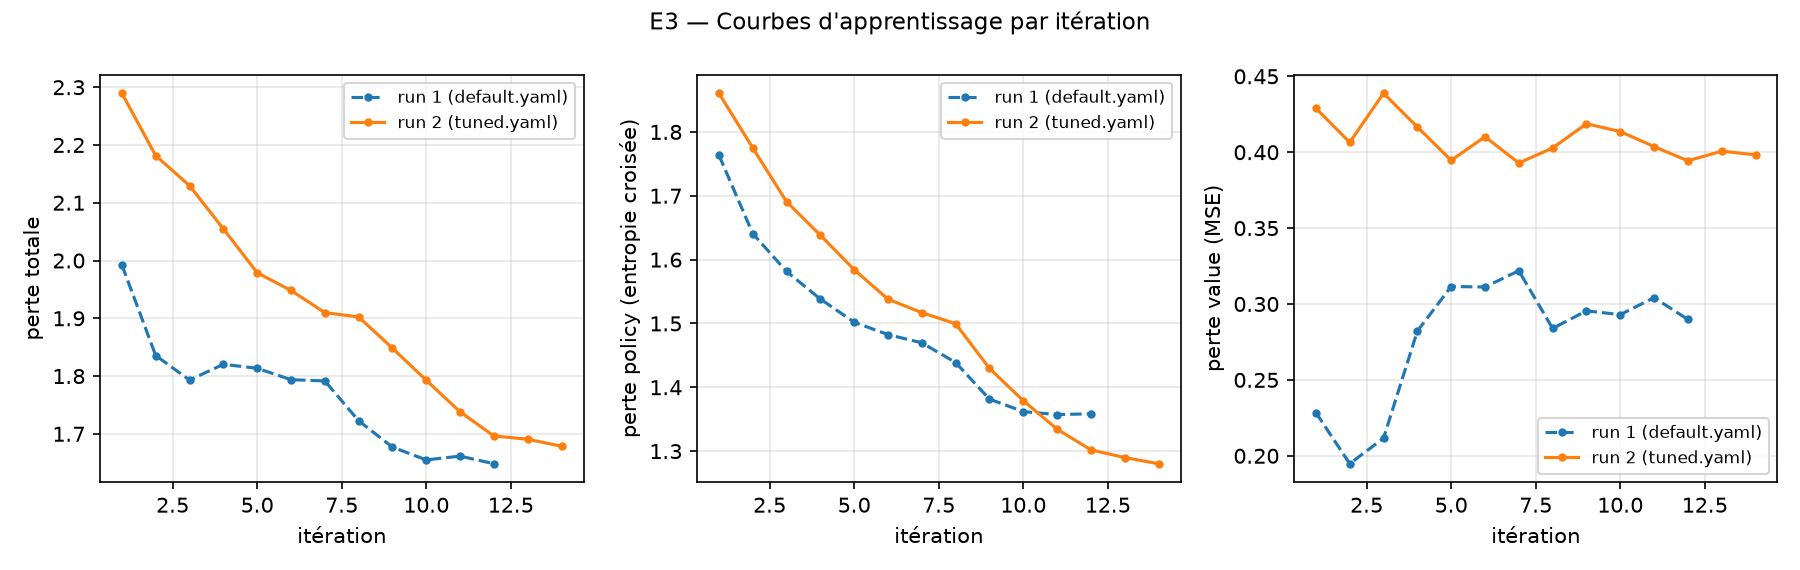
\includegraphics[width=0.74\linewidth]{figures/fig_E3_courbes_apprentissage.png}
\caption{E3 --- Perte totale, perte policy et perte value par itération, pour les deux runs.}
\end{figure}

La perte totale décroît dans les deux cas (run 1 : 1,992 $\rightarrow$ 1,648 ; run 2 : 2,290 $\rightarrow$
1,679), et la perte policy décroît régulièrement (run 2 : 1,861 $\rightarrow$ 1,280). \textbf{Le
critère C5 est atteint.}

Un point mérite d'être signalé : la \textbf{perte value
augmente} au cours du run 1 (0,228 $\rightarrow$ 0,290) et reste à peu près plate au run 2
(0,429 $\rightarrow$ 0,398). Ce n'est pas seulement un signe de sur-apprentissage : la
distribution des données change en cours de route, puisque les parties de
self-play s'allongent (1 776 échantillons à l'itération 1 du run 1, 1 984 à la
douzième) et deviennent moins triviales à évaluer. Une perte de value stable sur
des données qui se durcissent n'est pas la même chose qu'une perte de value qui
stagne à données fixes.

\subsection{Force au fil des itérations (E4)}\label{force-au-fil-des-ituxe9rations-e4}

\begin{figure}[htbp]
\centering
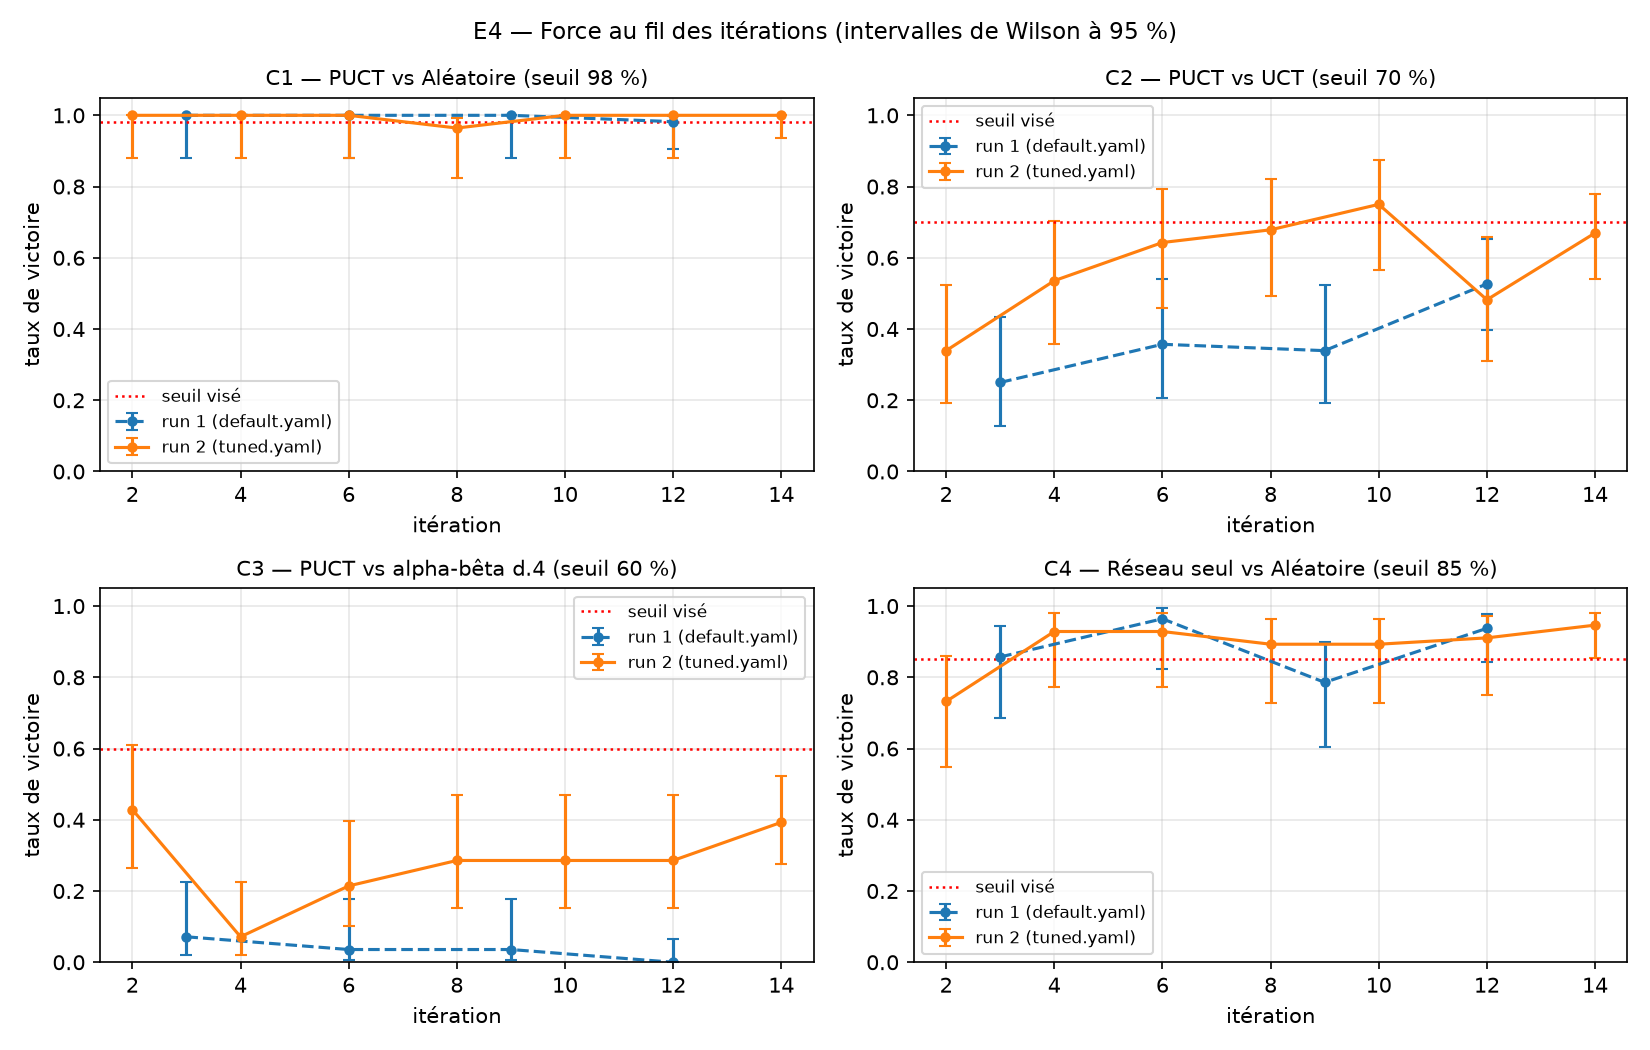
\includegraphics[width=0.72\linewidth]{figures/fig_E4_force_par_iteration.png}
\caption{E4 --- Les quatre critères mesurés tous les 2 ou 3 itérations, avec intervalles de Wilson à 95 \%. Le seuil visé est en pointillé rouge.}
\end{figure}

C1 (contre l'aléatoire) est saturé dès la première évaluation dans les deux runs.
C4, \textbf{le critère décisif}, monte à 94,6 \% au run 2. C2 progresse nettement au run 2
(33,9 \% $\rightarrow$ 75,0 \% à l'itération 10, 67,0 \% à la fin). C3 est le seul à rester loin
de son seuil, et c'est là que les deux runs divergent le plus violemment : le run 1
finit à \textbf{0,0 \%}, le run 2 à 39,3 \% sur le même protocole (puis 53,1 \% sur le
protocole corrigé de la §6).

La forte variabilité de C2 et C3 d'une évaluation à l'autre (C2 : 67,9 \% à
l'itération 8, 75,0 \% à la 10, 48,2 \% à la 12, 67,0 \% à la 14) rappelle que
28 parties donnent un intervalle de confiance d'environ $\pm$17 points. \textbf{Il ne faut
pas lire ces courbes coup par coup}, seulement leur tendance.

\subsection{Force en fonction du budget (E5) --- la figure centrale}\label{force-en-fonction-du-budget-e5-la-figure-centrale}

\begin{figure}[htbp]
\centering
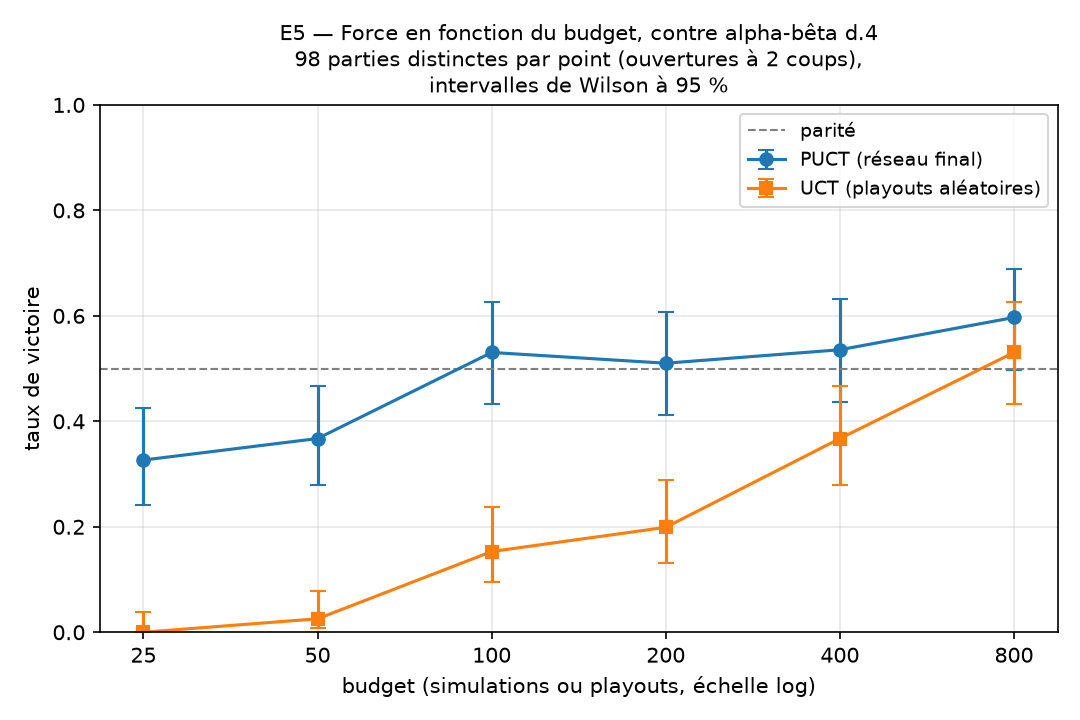
\includegraphics[width=0.44\linewidth]{figures/fig_E5_budget_simulations.png}
\caption{E5 --- Taux de victoire contre l'alpha-bêta de profondeur 4, en fonction du budget de simulations, échelle logarithmique. 98 parties distinctes par point.}
\end{figure}

\begin{table}[htbp]
\centering\small
\caption{E5 --- taux de victoire contre l'alpha-bêta de profondeur 4 selon le budget (98 parties distinctes par point).}
\label{tab:e5}
\begin{tabular}{@{}lcccccc@{}}
\toprule
\textbf{budget} & \textbf{25} & \textbf{50} & \textbf{100} & \textbf{200} & \textbf{400} & \textbf{800} \\
\midrule
\textbf{PUCT} (réseau final) & 32,7 \% & 36,7 \% & 53,1 \% & 51,0 \% & 53,6 \% & 59,7 \% \\
\textbf{UCT} (playouts aléatoires) & 0,0 \% & 2,6 \% & 15,3 \% & 19,9 \% & 36,7 \% & 53,1 \% \\
\bottomrule
\end{tabular}
\end{table}

\textbf{C'est la figure qui montre l'apport du réseau, et elle le montre sans ambiguïté.}
À budget égal, PUCT domine UCT partout, et l'écart est spectaculaire aux petits
budgets : à 25 simulations, PUCT obtient déjà 32,7 \% là où UCT ne gagne \textbf{aucune}
des 98 parties. La lecture la plus parlante est horizontale :

\begin{quote}
\textbf{PUCT à 100 simulations (53,1 \%) fait jeu égal avec UCT à 800 playouts
(53,1 \%).} Le réseau vaut donc, en première approximation, un facteur 8 sur le
budget de recherche.
\end{quote}

C'est exactement ce qu'on attend d'un prior appris : il dit à la recherche où
regarder, et évite de dépenser des simulations sur les six autres colonnes.

Deux réserves. D'abord, la comparaison est à \textbf{budget de simulations}
égal, pas à \textbf{temps} égal : une simulation PUCT coûte une passe réseau ($\approx$ 1 ms),
un playout UCT coûte une partie aléatoire ($\approx$ 0,03 ms). À temps égal, l'avantage de
PUCT disparaîtrait en grande partie. C'est la comparaison que fait le cours et
celle qui isole l'apport du réseau, mais il faut le dire. Ensuite, la courbe PUCT est
\textbf{plate entre 100 et 400 simulations} : la politique finale est très piquée
(0,914 sur la colonne centrale au plateau vide) et la recherche ne fait souvent que
confirmer le prior ; il faut passer à 800 pour qu'elle se remette à progresser.

\subsection{Accord avec le jeu parfait (E6)}\label{accord-avec-le-jeu-parfait-e6}

\begin{figure}[htbp]
\centering
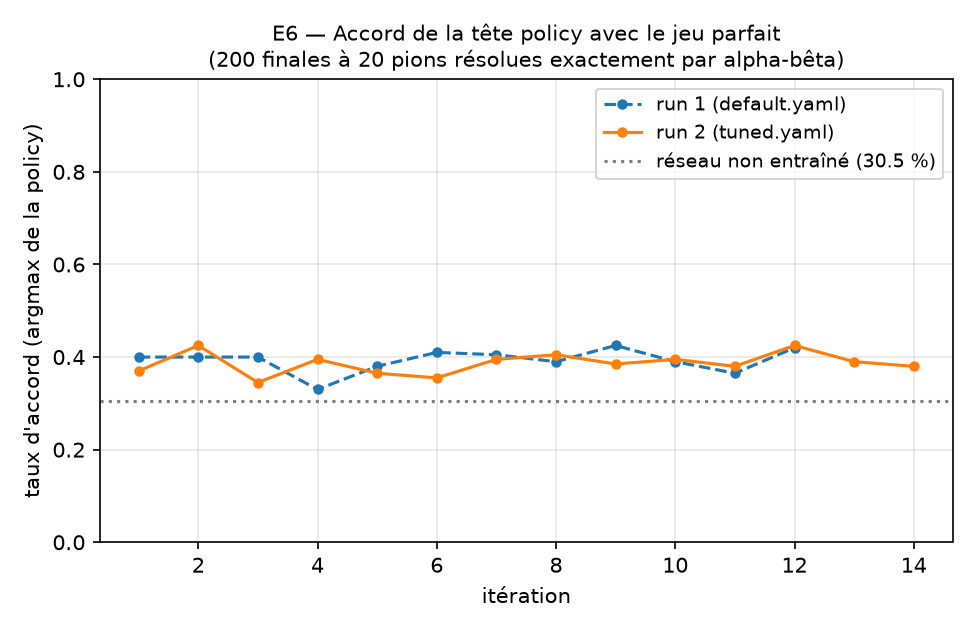
\includegraphics[width=0.44\linewidth]{figures/fig_E6_accord_jeu_parfait.png}
\caption{E6 --- Taux d'accord de l'argmax de la policy avec le jeu parfait, sur 200 finales à 20 pions résolues exactement.}
\end{figure}

Le réseau non entraîné (initialisé à graine fixe) est à 30,5 \%, et un agent qui
jouerait au hasard serait à environ 25 \%. Dès la première itération, la policy
monte à 37--40 \%, puis \textbf{plafonne} : elle oscille entre 34,5 \% et 42,5 \% pendant
tout le reste de l'entraînement, dans les deux runs.

C'est un résultat en demi-teinte qu'il faut prendre pour ce qu'il est : le réseau
apprend très vite une heuristique positionnelle utile (jouer au centre, empiler,
compléter un alignement), qui lui fait gagner une dizaine de points d'accord avec
le jeu parfait, mais il \textbf{n'apprend pas à résoudre les finales}. Ce n'est pas surprenant : une finale à
20 pions se gagne par un calcul tactique exact sur une dizaine de coups, ce qu'une
politique sans recherche ne peut pas faire, et ce que 1 300 parties de self-play ne
suffisent certainement pas à lui apprendre. Cette métrique est celle qui montre le
plus clairement la limite de notre budget de calcul.

\subsection{Le réseau redécouvre la colonne centrale (E7)}\label{le-ruxe9seau-reduxe9couvre-la-colonne-centrale-e7}

\begin{figure}[htbp]
\centering
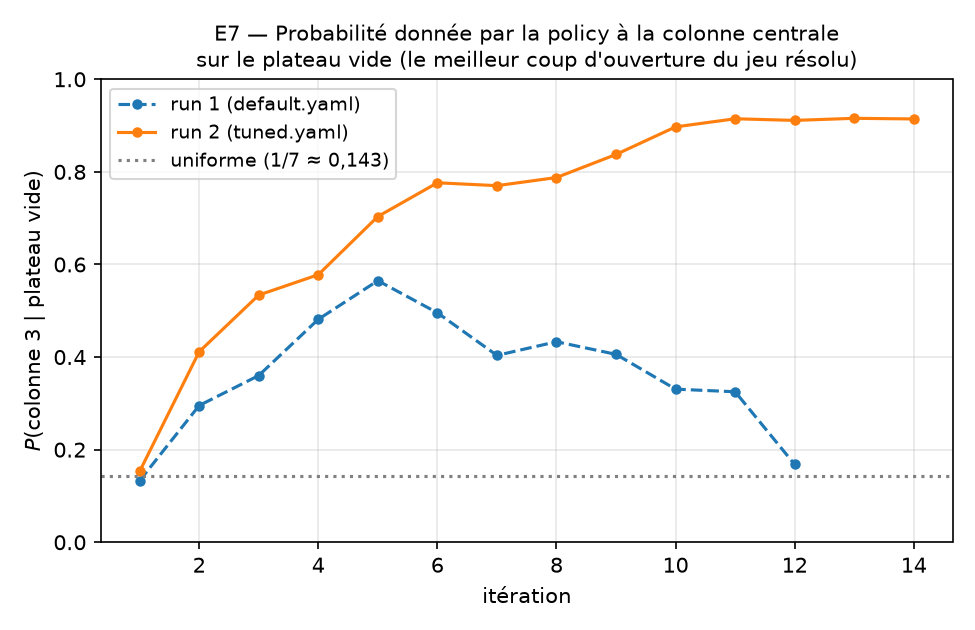
\includegraphics[width=0.44\linewidth]{figures/fig_E7_prior_colonne_centrale.png}
\caption{E7 --- Probabilité donnée par la tête policy à la colonne centrale sur le plateau vide, par itération.}
\end{figure}

\textbf{C'est le plus beau résultat du projet.} Le Puissance 4 est un jeu résolu et l'on
sait que \textbf{le coup d'ouverture optimal est la colonne centrale}. Or notre réseau
ne dispose d'aucune connaissance experte : ni ouvertures, ni heuristique, ni la
moindre indication qu'une colonne vaudrait mieux qu'une autre. Il part d'une
politique quasi uniforme (0,153 $\approx$ 1/7 à l'itération 1).

Au run 2, la probabilité de la colonne centrale monte \textbf{de façon monotone} :
0,153 $\rightarrow$ 0,412 $\rightarrow$ 0,534 $\rightarrow$ 0,578 $\rightarrow$ 0,701 $\rightarrow$ 0,775 $\rightarrow$ \ldots{} $\rightarrow$ \textbf{0,914} à la quatorzième
itération. Le réseau a donc \textbf{redécouvert tout seul, par pur self-play, un
résultat connu du jeu résolu.}

La courbe du run 1 est tout aussi parlante, dans l'autre sens : elle monte à 0,563
à l'itération 5, puis \textbf{s'effondre} jusqu'à 0,168 --- c'est-à-dire pratiquement le
niveau uniforme. C'est la signature visuelle de l'effondrement analysé en §8.

\section{Discussion et limites}
\label{sec:discussion}

\subsection{Le run 1 : anatomie d'un échec}\label{le-run-1-anatomie-dun-uxe9chec}

Le run 1 utilisait la configuration initiale (\texttt{default.yaml} :
12 itérations $\times$ 40 parties $\times$ 300 pas). Il a échoué franchement : C2 à 52,7 \% et
\textbf{C3 à 0,0 \%} --- PUCT ne gagnait littéralement aucune partie contre l'alpha-bêta.

Nous avons suivi une liste de contrôle, dans l'ordre, avant de toucher à
quoi que ce soit :

\begin{enumerate}
\def\labelenumi{\arabic{enumi}.}
\setlength{\itemsep}{1pt}\setlength{\parskip}{0pt}
\item
  \textbf{le réseau sait-il sur-apprendre 100 échantillons ?} Oui : $\mathrm{KL} = 2\cdot 10^{-5}$,
  $\mathrm{MSE} = 1\cdot 10^{-5}$. (Au passage, notre première version de ce test échouait avec une
  MSE bloquée à 0,0428 ; l'explication était que le jeu de test contenait 6
  positions dupliquées portant des cibles aléatoires contradictoires, et 0,0428
  était \textbf{exactement} la variance intra-groupe irréductible. Le réseau était
  parfait, le jeu de données ne l'était pas.)
\item
  \textbf{le signe de \texttt{z} ?} Vérifié par le test sur vérité terrain exacte (§5.4).
\item
  \textbf{$\pi$ calculé après le bruit ?} Oui.
\item
  \textbf{la symétrie appliquée aux plans \emph{et} à $\pi$ ?} Oui.
\item
  \textbf{le budget d'entraînement ?} C'est là qu'était le problème.
\end{enumerate}

Le diagnostic décisif a été de mesurer, \textbf{checkpoint par checkpoint}, la tactique
élémentaire de PUCT et la saturation de la tête value :

\begin{table}[htbp]
\centering\small
\caption{Diagnostic du run 1, checkpoint par checkpoint. « value saturée » est la proportion de positions où la tête value sort exactement $\pm 1$.}
\label{tab:diagnostic}
\begin{tabular}{@{}lccccc@{}}
\toprule
\textbf{checkpoint} & \textbf{value saturée} & \textbf{écart-type de $v$} & \textbf{gains pris /30} & \textbf{parades /30} & \textbf{accord policy} \\
\midrule
non entraîné & 0,0 \% & 0,003 & \textbf{30} & \textbf{30} & 30,5 \% \\
iter 03 & 6,0 \% & 0,760 & 25 & 24 & 40,0 \% \\
iter 06 & \textbf{13,0 \%} & 0,803 & \textbf{22} & \textbf{20} & 41,0 \% \\
iter 09 & 13,0 \% & 0,782 & 25 & 24 & 42,5 \% \\
iter 12 & 9,7 \% & 0,752 & 24 & 24 & 42,0 \% \\
\bottomrule
\end{tabular}
\end{table}

\begin{figure}[htbp]
\centering
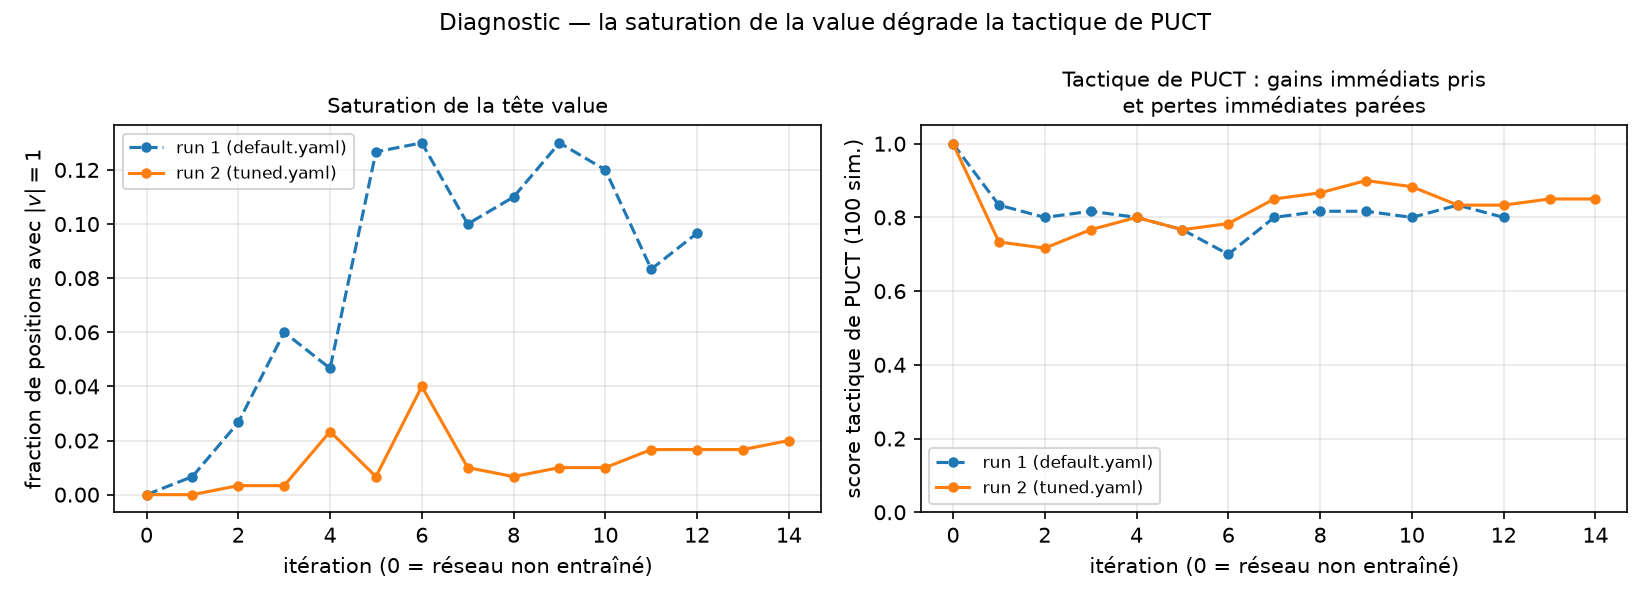
\includegraphics[width=0.74\linewidth]{figures/fig_diagnostic_saturation.png}
\caption{Diagnostic --- la saturation de la tête value et la dégradation de la tactique de PUCT, pour les deux runs.}
\end{figure}

Le constat est brutal : \textbf{le réseau non entraîné donne une tactique parfaite
(30/30 et 30/30), et l'entraînement la dégrade} jusqu'à 22/30 et 20/30. Plus on
entraîne, moins PUCT sait prendre un gain immédiat.

Le mécanisme est le suivant. La tête value \textbf{sature} : sur 13 \% des positions
elle sort exactement $\pm$1. Or dans PUCT, une feuille terminale gagnante remonte
\texttt{score()\ =\ 1}, et une feuille non terminale que le réseau juge gagnante remonte
elle aussi une valeur de 1. \textbf{Les deux deviennent indiscernables.} Le $Q$ du vrai
gain immédiat et celui d'un coup quelconque que le réseau surestime sont égaux, et
le départage se fait alors sur le terme $c_{\mathrm{puct}}P(a{\mid}s)\sqrt{N}/(1+N(s,a))$,
c'est-à-dire \textbf{sur le prior}. Si la policy préfère un autre coup, la recherche
suit la policy et rate le gain. Le réseau non entraîné, dont la value est
quasi constante à --0,16 (écart-type 0,012), n'a pas ce problème : la valeur
terminale 1 domine toujours strictement.

La cause racine est un \textbf{sur-apprentissage} : 300 pas de gradient de taille 128 sur
environ 1 900 échantillons frais, cela fait à peu près \textbf{20 époques par itération}
sur les données les plus récentes. Les deux têtes mémorisent, la value sature sur
des cibles $\pm$1, et comme les cibles de self-play sont produites \emph{par cette même
recherche dégradée}, la boucle se referme : mauvaise recherche $\rightarrow$ mauvaises cibles $\rightarrow$
mauvais réseau. La courbe E7 du run 1 (montée à 0,56 puis effondrement à 0,17) est
la même histoire vue depuis la policy.

\subsection{Le run 2 : la correction et ce qu'elle a donné}\label{le-run-2-la-correction-et-ce-quelle-a-donnuxe9}

Nous avons changé \textbf{une seule chose}, dictée par le diagnostic : le rapport entre
la quantité de données et le nombre de pas de gradient. 96 parties par itération au
lieu de 40, 200 pas au lieu de 300 --- soit environ \textbf{6 époques} de données fraîches
au lieu de 20.

Le résultat valide le diagnostic :

\begin{table}[htbp]
\centering\small
\caption{Effet de la correction apportée au run 2.}
\label{tab:run2}
\begin{tabular}{@{}lll@{}}
\toprule
& run 1 & run 2 \\
\midrule
saturation maximale de la value & 13,0 \% & \textbf{4,0 \%} \\
tactique finale (gains / parades sur 30) & 24 / 24 & \textbf{26 / 25} \\
$P(\text{centre})$ finale & 0,168 (effondrée) & \textbf{0,914} \\
C2 & 52,7 \% & 67,0 \% \\
C3 & 0,0 \% & 39,3 \% (53,1 \% protocole corrigé) \\
\bottomrule
\end{tabular}
\end{table}

La saturation est divisée par trois, l'effondrement de la policy disparaît, et C3
passe de 0 \% à un score autour de la parité. \textbf{Nous avons donc bien retiré la cause,
pas le symptôme.}

\subsection{Ce qui n'est toujours pas résolu}\label{ce-qui-nest-toujours-pas-ruxe9solu}

Il faut le dire clairement : \textbf{PUCT reste tactiquement inférieur au réseau non
entraîné} (26/30 contre 30/30 sur les gains immédiats). La saturation est réduite,
pas supprimée. Une tête value entraînée avec une MSE sur des cibles $\pm$1 tend
naturellement vers la saturation, et c'est structurel. Les remèdes usuels
(beaucoup plus de parties, ou traiter explicitement les nœuds terminaux dans la
recherche) sortent du périmètre que nous nous étions fixé : le second est un
\textbf{MCTS Solver}, que nous listons en §9 parmi les techniques du cours non
implémentées, et c'est très exactement le problème qu'il résout.

C'est la raison pour laquelle C2 et C3 ne sont pas atteints. Nous ne pensons pas
que ce soit un défaut d'implémentation : c'est le budget de calcul. 1 344 parties
de self-play, c'est deux ordres de grandeur en dessous de ce qu'un AlphaZero pour
Puissance 4 utilise habituellement.

\subsection{Variance des mesures}\label{variance-des-mesures}

Avec 28 parties, l'intervalle de Wilson fait environ $\pm$17 points ; avec 98, environ
$\pm$10. Beaucoup de nos comparaisons ne sont donc \textbf{pas} significatives, et nous
l'avons signalé à chaque fois plutôt que de commenter du bruit : la grille de
constantes d'exploration E2 (sauf pour \texttt{c\ =\ 1,0}), l'écart Flat MC / UCB en E1, et
GRAVE vs UCT à 200 playouts sont tous dans ce cas. Les résultats que nous
considérons comme établis sont ceux dont l'intervalle exclut le seuil discuté :
UCT \textgreater{} Flat MC et UCT \textgreater{} UCB (E1), PUCT \textgreater{} UCT à tous les budgets (E5), GRAVE \textless{} UCT à
1 000 playouts (E8), C1 et C4.

\subsection{Coût de calcul}\label{couxfbt-de-calcul}

Le projet entier --- deux entraînements, le test set résolu exactement, les neuf
expériences et le diagnostic --- tient en \textbf{environ 50 minutes de CPU} sur une
machine à 8 cœurs. La parallélisation racine du self-play sur 6 workers est ce qui
rend cela possible.

\section{Perspectives : les techniques du cours que nous n'avons pas implémentées}\label{perspectives-les-techniques-du-cours-que-nous-navons-pas-impluxe9mentuxe9es}

Cette section liste les techniques présentées dans le cours et laissées de côté,
avec pour chacune ce qu'elle fait et pourquoi elle était hors périmètre.

\begin{itemize}
\item
  \textbf{MCTS Solver / Score Bounded MCTS} --- propagent dans l'arbre l'information
  « cette position est \emph{prouvée} gagnée / perdue » au lieu d'une moyenne, ce qui
  permet de couper les branches résolues et de jouer parfaitement les finales.
  C'est, rétrospectivement, \textbf{la technique du cours qui aurait le plus servi ici} :
  la §8.3 montre que notre problème résiduel est précisément qu'une feuille
  terminale gagnante et une feuille que la value surestime deviennent
  indiscernables, ce qu'un solveur règle par construction. Nous l'avions écartée en
  jugeant qu'à 100 simulations sur un branchement de 7 la recherche couvrait déjà
  bien les tactiques ; le diagnostic montre que ce jugement était le mauvais.
\item
  \textbf{Sequential Halving}~\cite{karnin2013}, et ses versions en arbre
  \textbf{SHOT}~\cite{cazenave2015shot} et \textbf{SHUSS}~\cite{fabiano2019} ---
  éliminent à chaque tour la moitié des coups les moins prometteurs, ce qui donne
  à la racine une garantie de \emph{simple regret} que UCB n'offre pas ; SHUSS y
  ajoute un biais fondé sur les statistiques AMAF. C'est une ablation sur
  l'allocation du budget, qui ne change pas la démonstration portant sur l'apport
  du réseau --- et le biais AMAF de SHUSS tient de toute façon mal au Puissance 4
  (§3.7).
\item
  \textbf{PPA / PPAF}~\cite{cazenave2016ppa}, \textbf{Nested Monte Carlo
  Search}~\cite{cazenave2009} et \textbf{NRPA}~\cite{rosin2011nrpa} --- respectivement :
  apprendre en ligne une politique de playout paramétrée par les codes de coups,
  choisir chaque coup par une recherche de niveau inférieur, et combiner les deux
  par gradient. Ce sont les méthodes de référence sur les problèmes
  d'optimisation à un joueur (Morpion Solitaire, SameGame) ; elles supposent en
  outre des codes de coups porteurs de signal --- la même faiblesse qu'AMAF ici.
\item
  \textbf{Descent / minimax non borné (Athénan)}~\cite{cohensolal2020},
  \textbf{MuZero}~\cite{schrittwieser2020} et \textbf{Polygames}~\cite{cazenave2020} ---
  remonter un minimax dans l'arbre partiel plutôt qu'une moyenne ; apprendre
  \emph{en plus} la dynamique du jeu pour planifier dans un espace latent ; généraliser
  AlphaZero à des plateaux de taille variable. Hors périmètre d'un projet de TP,
  et sans objet ici : nous connaissons les règles, et la grille est fixée à 6$\times$7.
\item
  \textbf{Parallélisation d'arbre (avec verrous ou \emph{lock-free})} --- plusieurs threads
  descendent le \emph{même} arbre, ce qui partage l'information mais demande des
  précautions de concurrence (et typiquement une \emph{virtual loss}). Nous avons choisi
  la \textbf{parallélisation racine}, celle du cours qui demande le moins de machinerie,
  et qui suffit largement puisque nos processus jouent des parties entières
  indépendantes.
\end{itemize}

Enfin, et \textbf{hors du cours donc exclues par principe} : bitboards (§5.6),
\emph{virtual loss}, Gumbel AlphaZero, mécanisme de \emph{resign}, inférence batchée. Sur ce
dernier point, notons que la mise en cache du prior et de la value dans l'entrée de
la table de transposition fait que chaque position distincte n'est évaluée qu'une
seule fois par recherche : avec un taux de hit de 78,4 \%, le batching aurait peu à
récupérer.

\section{Conclusion}
\label{sec:conclusion}

Les cinq barreaux de l'échelle du cours sont implémentés, du playout aléatoire à
l'AlphaZero miniature. Trois critères sur cinq sont atteints, dont \textbf{C4, le critère décisif} : à zéro
simulation, la seule tête policy bat l'aléatoire 93,8 \% du temps, ce qui prouve que
le réseau a appris. Deux résultats nous paraissent valoir plus que les taux de
victoire eux-mêmes :

\begin{itemize}
\setlength{\itemsep}{1pt}\setlength{\parskip}{0pt}
\item
  \textbf{E5} quantifie l'apport du réseau : PUCT à 100 simulations vaut UCT à
  800 playouts, un facteur 8 sur le budget de recherche ;
\item
  \textbf{E7} montre le réseau redécouvrir seul, par pur self-play et sans aucune
  connaissance experte, que la colonne centrale est le meilleur coup d'ouverture ---
  un résultat connu du jeu résolu, atteint avec une probabilité de 0,914.
\end{itemize}

Les deux critères manqués (C2 et C3) le sont pour une raison identifiée et
mesurée : la saturation de la tête
value dégrade la tactique de PUCT, et c'est un manque de données de self-play, pas
un défaut de l'implémentation. Le remède le plus direct dans le périmètre du cours
serait un \textbf{MCTS Solver}.

\begin{thebibliography}{99}
\footnotesize\setlength{\itemsep}{0pt}\setlength{\parskip}{0pt}

\bibitem{cazenave-cours} T.~Cazenave.
  \emph{Monte Carlo Search}. Support de cours, Université Paris Dauphine -- PSL.
  (Source principale de ce projet ; les travaux ci-dessous sont ceux qu'il cite.)

\bibitem{allis1988} L.~V. Allis.
  \emph{A Knowledge-based Approach of Connect-Four}.
  Mémoire, Vrije Universiteit Amsterdam, 1988.

\bibitem{allen1989} J.~D. Allen.
  \emph{A Note on the Computer Solution of Connect-Four}. 1989.

\bibitem{brugmann1993} B.~Brügmann.
  \emph{Monte Carlo Go}. Rapport technique, 1993.

\bibitem{kocsis2006} L.~Kocsis et C.~Szepesvári.
  \emph{Bandit based Monte-Carlo Planning}. ECML, pages 282--293, 2006.

\bibitem{gelly2007} S.~Gelly et D.~Silver.
  \emph{Combining Online and Offline Knowledge in UCT}. ICML, pages 273--280, 2007.
  (RAVE)

\bibitem{cazenave2015grave} T.~Cazenave.
  \emph{Generalized Rapid Action Value Estimation}. IJCAI, pages 754--760, 2015.
  (GRAVE)

\bibitem{rosin2011puct} C.~D. Rosin.
  \emph{Multi-armed Bandits with Episode Context}.
  Annals of Mathematics and Artificial Intelligence, 61(3):203--230, 2011.
  (la formule PUCT)

\bibitem{silver2016} D.~Silver et al.
  \emph{Mastering the Game of Go with Deep Neural Networks and Tree Search}.
  Nature, 529:484--489, 2016. (AlphaGo)

\bibitem{silver2017} D.~Silver et al.
  \emph{Mastering the Game of Go without Human Knowledge}.
  Nature, 550:354--359, 2017. (AlphaGo Zero)

\bibitem{silver2018} D.~Silver et al.
  \emph{A General Reinforcement Learning Algorithm that Masters Chess, Shogi and Go
  through Self-Play}. Science, 362:1140--1144, 2018. (AlphaZero)

\bibitem{schrittwieser2020} J.~Schrittwieser et al.
  \emph{Mastering Atari, Go, Chess and Shogi by Planning with a Learned Model}.
  Nature, 588:604--609, 2020. (MuZero)

\bibitem{karnin2013} Z.~Karnin, T.~Koren et O.~Somekh.
  \emph{Almost Optimal Exploration in Multi-Armed Bandits}. ICML, 2013.
  (Sequential Halving)

\bibitem{cazenave2015shot} T.~Cazenave.
  \emph{Sequential Halving Applied to Trees}. IEEE TCIAIG, 7(1):102--105, 2015.

\bibitem{fabiano2019} N.~Fabiano et T.~Cazenave.
  \emph{Sequential Halving Using Scores}. ACG, 2019. (SHUSS)

\bibitem{cazenave2009} T.~Cazenave.
  \emph{Nested Monte-Carlo Search}. IJCAI, pages 456--461, 2009.

\bibitem{rosin2011nrpa} C.~D. Rosin.
  \emph{Nested Rollout Policy Adaptation for Monte Carlo Tree Search}.
  IJCAI, pages 649--654, 2011.

\bibitem{cazenave2016ppa} T.~Cazenave.
  \emph{Playout Policy Adaptation for Games}. ACG, 2016.

\bibitem{cohensolal2020} Q.~Cohen-Solal.
  \emph{Learning to Play Two-Player Perfect-Information Games without Knowledge}.
  2020. (Descent, Athénan)

\bibitem{cazenave2020} T.~Cazenave et al.
  \emph{Polygames: Improved Zero Learning}. ICGA Journal, 42(4):244--256, 2020.

\bibitem{zobrist1970} A.~L. Zobrist.
  \emph{A New Hashing Method with Application for Game Playing}.
  Rapport technique, University of Wisconsin, 1970.

\bibitem{wilson1927} E.~B. Wilson.
  \emph{Probable Inference, the Law of Succession, and Statistical Inference}.
  Journal of the American Statistical Association, 22:209--212, 1927.

\end{thebibliography}

\appendix

\section{Reproduire les résultats}
\label{sec:repro}

\begin{lstlisting}[language=bash,caption={Commandes.},numbers=none]
python3 -m venv .venv && source .venv/bin/activate
pip install -r requirements.txt
python -m pytest -q                       # tests
python main.py testset --n 200 --min-stones 20   # finales resolues exactement
python main.py pipeline --config configs/default.yaml \
       --log report/results/training_log_run1.jsonl   # run 1  (~15 min)
python main.py pipeline --config configs/tuned.yaml \
       --log report/results/training_log_run2.jsonl   # run 2  (~20 min)
python scripts/run_experiments.py --workers 6 --k 4   # E1-E9, C1-C4 (~10 min)
python scripts/make_figures.py            # figures + tableaux
\end{lstlisting}

\textbf{Aucun chiffre de ce rapport n'est écrit à la main.} Tous proviennent des
fichiers JSON de \texttt{report/results/}, produits par
\texttt{run\_experiments.py} et mis en forme par \texttt{make\_figures.py}. Toutes
les expériences utilisent la graine \texttt{20260731}.

\section{Organisation du code}

\begin{center}
\footnotesize
\begin{tabular}{@{}ll@{}}
\toprule
Fichier & Rôle \\
\midrule
\texttt{game/connect4.py} & état, coups, Zobrist, symétrie, codes AMAF \\
\texttt{search/tt.py} & table de transposition \\
\texttt{search/flat.py}, \texttt{uct.py} & Flat MC, UCB à la racine, UCT récursif \\
\texttt{search/grave.py} & playoutAMAF, updateAMAF, RAVE, GRAVE \\
\texttt{search/puct.py} & PUCT guidé par le réseau \\
\texttt{model/} & encodage, \texttt{to\_pov}, symétrie, réseau à deux têtes \\
\texttt{train/} & self-play, buffer, entraînement, pipeline \\
\texttt{eval/} & arène, alpha-bêta, test set de finales \\
\texttt{scripts/} & expériences, figures, tableaux \\
\texttt{main.py} & ligne de commande \\
\bottomrule
\end{tabular}
\end{center}

\end{document}
